% !TEX root = main.tex
\section{Measurements and Verification}
\label{sec:verification}
In this section we present measurements and verifications of the proposed system. We first present a verification of the system specifications in section \ref{sec:specs_verification}. In section \ref{sec:perf_meas} the system performance will be evaluated under different conditions, and some key performance parameters will be presented.

\subsection{Verification of System Parameters}
\label{sec:specs_verification}
The verified system specifications is summarised in table \ref{tab:meas_specs}.
% !TEX root = main.tex
\begin{table}[htbp]
  \centering
  \caption{Summarised Measurements of System Parameters}
    \begin{tabular}{lc}
    \rowcolor[rgb]{ 0,  0,  0} \textcolor[rgb]{ 1,  1,  1}{\textbf{System Parameter}}	& \textcolor[rgb]{ 1,  1,  1}{\textbf{Measured Value}} 		\\
    	Half-Power Bandwidth										& \SI{\measBW}{kHz}					\\
    	PA power, $P_{PA}$ 											& \SI{\measPWR}{dBm}					\\
    	Delay 													& \SI{\measDelay}{ms} 					\\
 \end{tabular}
  \label{tab:meas_specs}
\end{table}

The power spectrum of the signal was analyzed in MATLAB's signal analyzer toolbox \cite{signalAnalyzer}. The baseband power spectrum is shown in figure \ref{fig:pwr_spectrum} together with the theoretical spectrum. The -40dBc bandwidth is measured to $\measBW \si{kHz}$.
The transmit power was verified by first calibrating the USRP power spectral density using a spectrum analyser, and then calculating the total transmit power from measured bandwidth\footnote{Due to the CIVID-19 situation the lab equipment was not available for measurements on the implemented system}. This way, the transmit power was measured to $\measPWR \si{dBm}$.

\begin{figure}[htbp]
\begin{center}
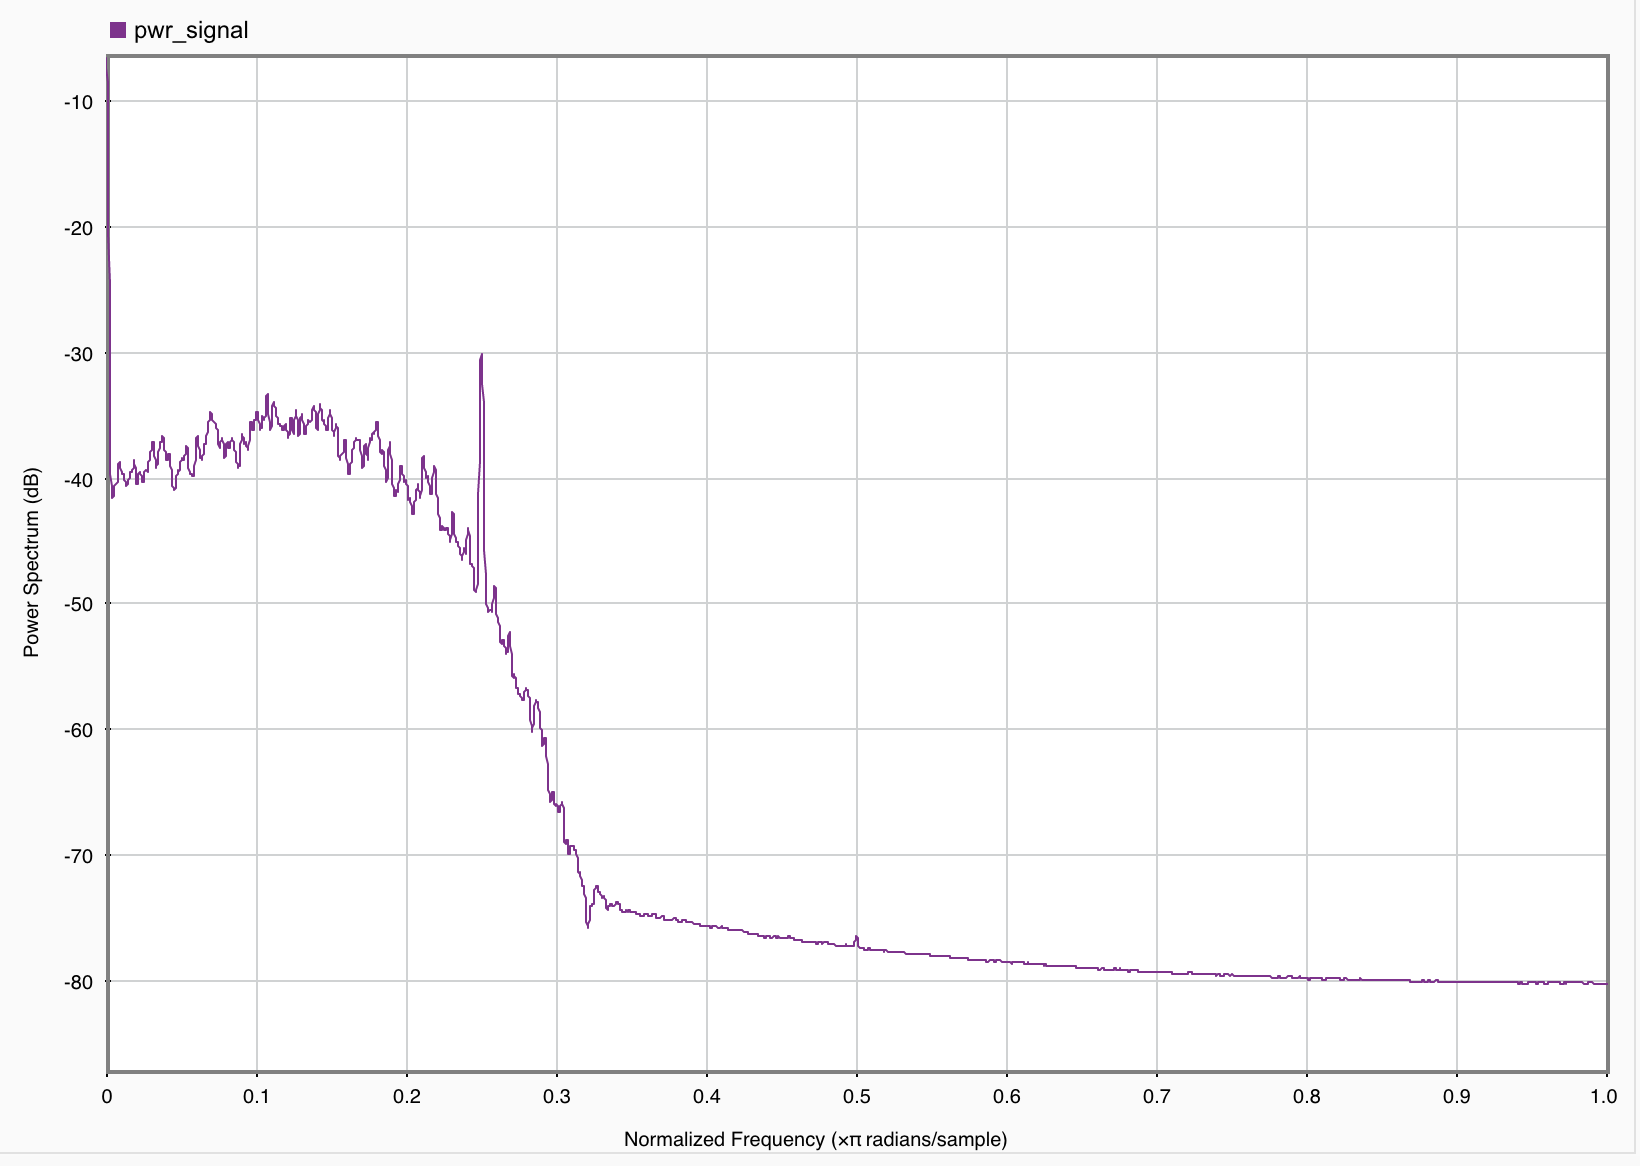
\includegraphics[width=\figW\linewidth]{spectrum.png}
\caption{Received signal power spectrum}
\label{fig:pwr_spectrum}
\end{center}
\end{figure}

The system delay was measured by transmitting a known bit sequence and evaluating the time delay from sound producer to sound consumer. The delay was measured by running both the transmitter and receiver software on the same computer. The average measured delay was $\measDelay \si{ms}$ with a sample standard deviation of $\measDelayStd \si{ms}$. 200ms of this delay originates from the buffers of the USRP.

\subsection{Performance Measurements}
\label{sec:perf_meas}
The system is tested in an indoor environment with both USRP's at the same height, 1 meter apart and no polarization mismatch\footnote{The measurements had to be performed in a tiny student apartment because the lab was closed}. For the sake of reproducibility, we chose to simulate the varying state of the radio channel by adjusting the transmit power instead of changing the radio channel physically. Two different transmit power levels was used to verify transmission at both qualities. High quality transmission was measured with a transmit power of $\measPWR \si{dBm}$ and low quality with $\measPWRbad \si{dBm}$. 

Eye diagram and constellation diagram is provided for both transmit power levels and both modulation formats, together with some key performance measurements. The diagrams for high and low transmit power are summarised in figure \ref{fig:good_diagrams} and \ref{fig:bad_diagrams} respectively. Estimated performance parameters are summarised in table \ref{tab:meas_params_good} and \ref{tab:meas_params_bad} for high and low transmit power respectively. In the tables, BER is the true measured bit error rate and error vector magnitude (EVM) and SNR is estimated from the constellation diagrams. EVM is the average magnitude of the error vector normalized to the peak constellation power. \ebnot is estimated using the measured -40dBc bandwidth for noise power.

% !TEX root = main.tex
\begin{figure} 
    \centering
  \subfloat[QPSK constellation\label{1a}]{%
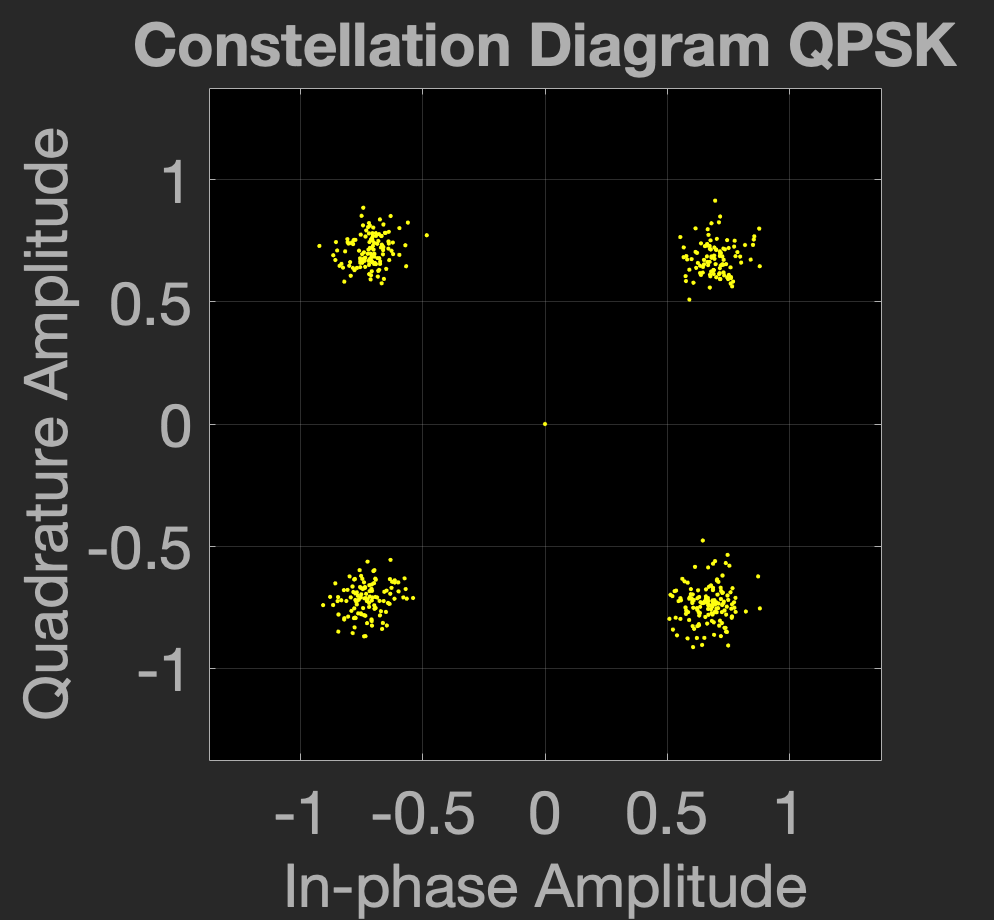
\includegraphics[width=0.45\linewidth]{constellationQPSKgood.png}
}
  \subfloat[QAM-16 constellation\label{1b}]{%
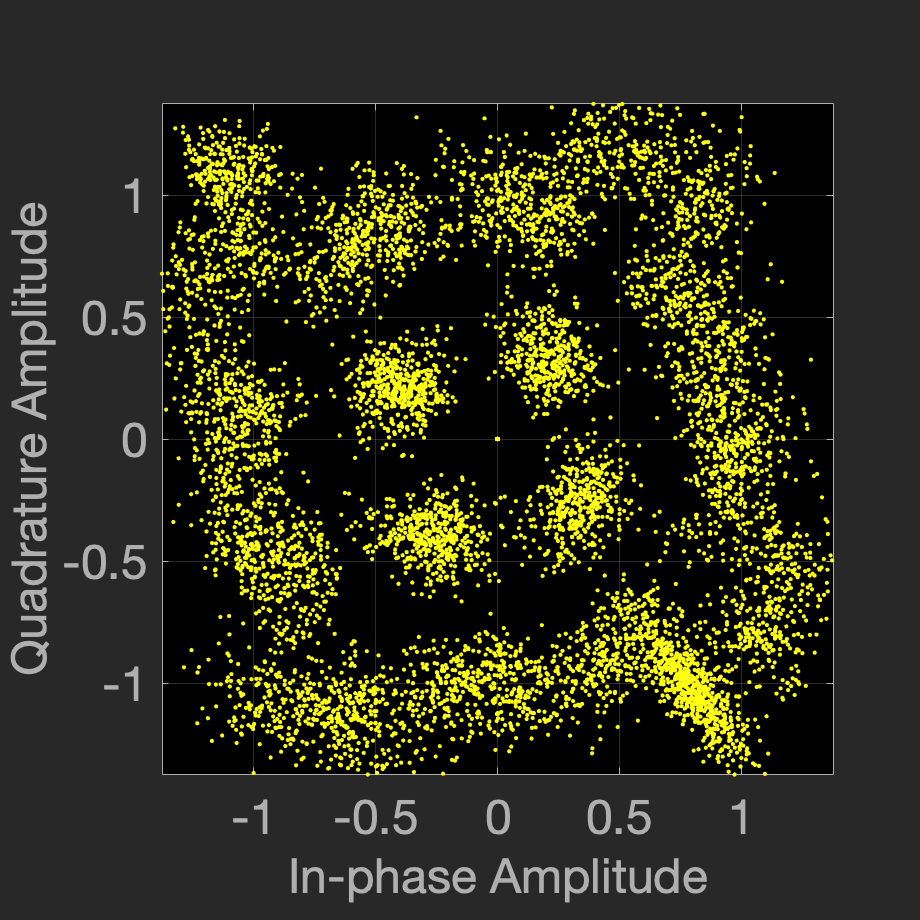
\includegraphics[width=0.45\linewidth]{constellationQAMgood.png}

}
\\
  \subfloat[QPSK eye diagram\label{1c}]{%
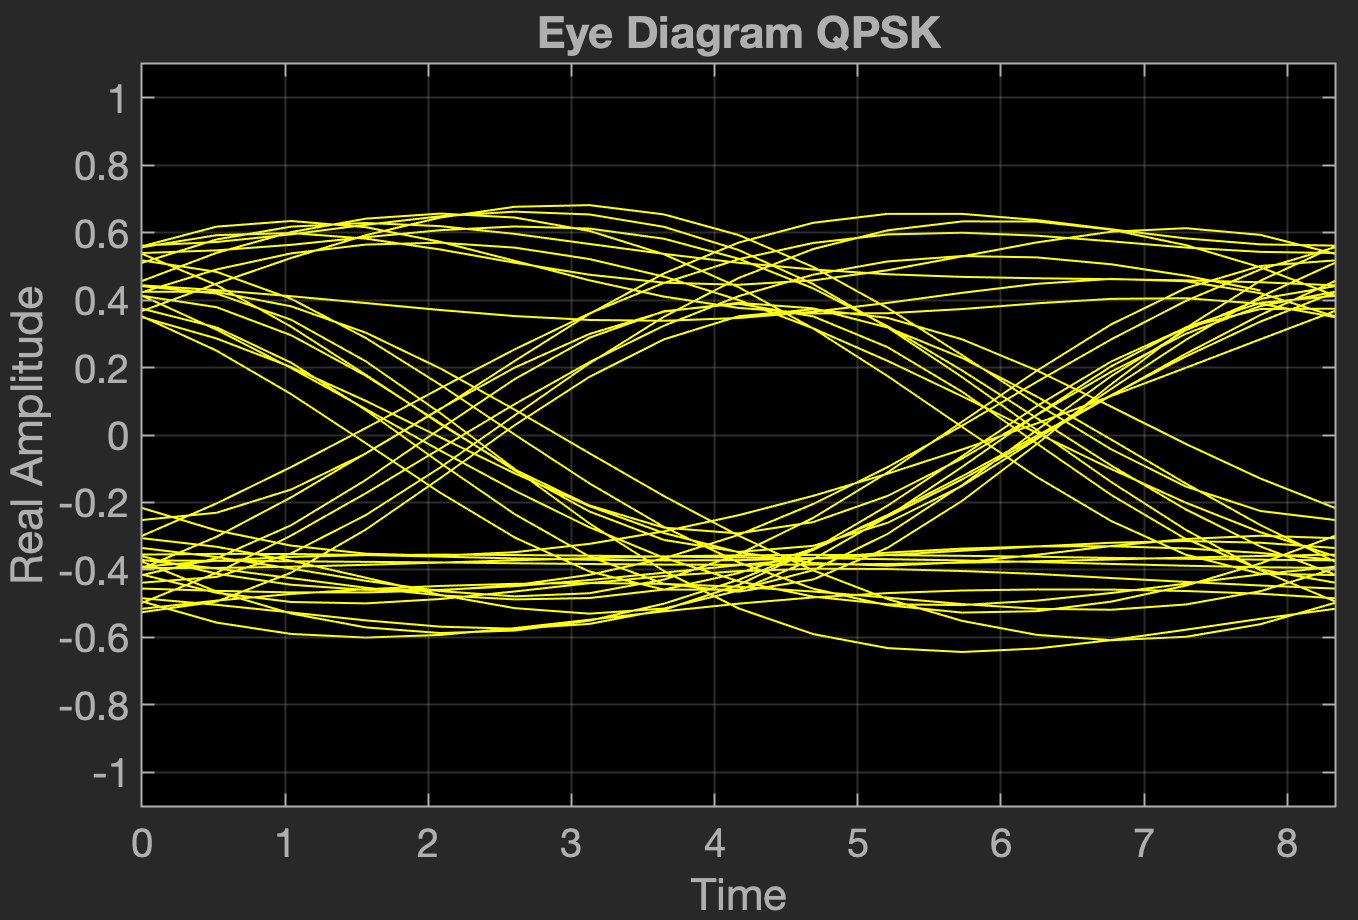
\includegraphics[width=0.45\linewidth]{eyeQPSKgood.png}

}
  \subfloat[QAM-16 eye diagram\label{1d}]{%
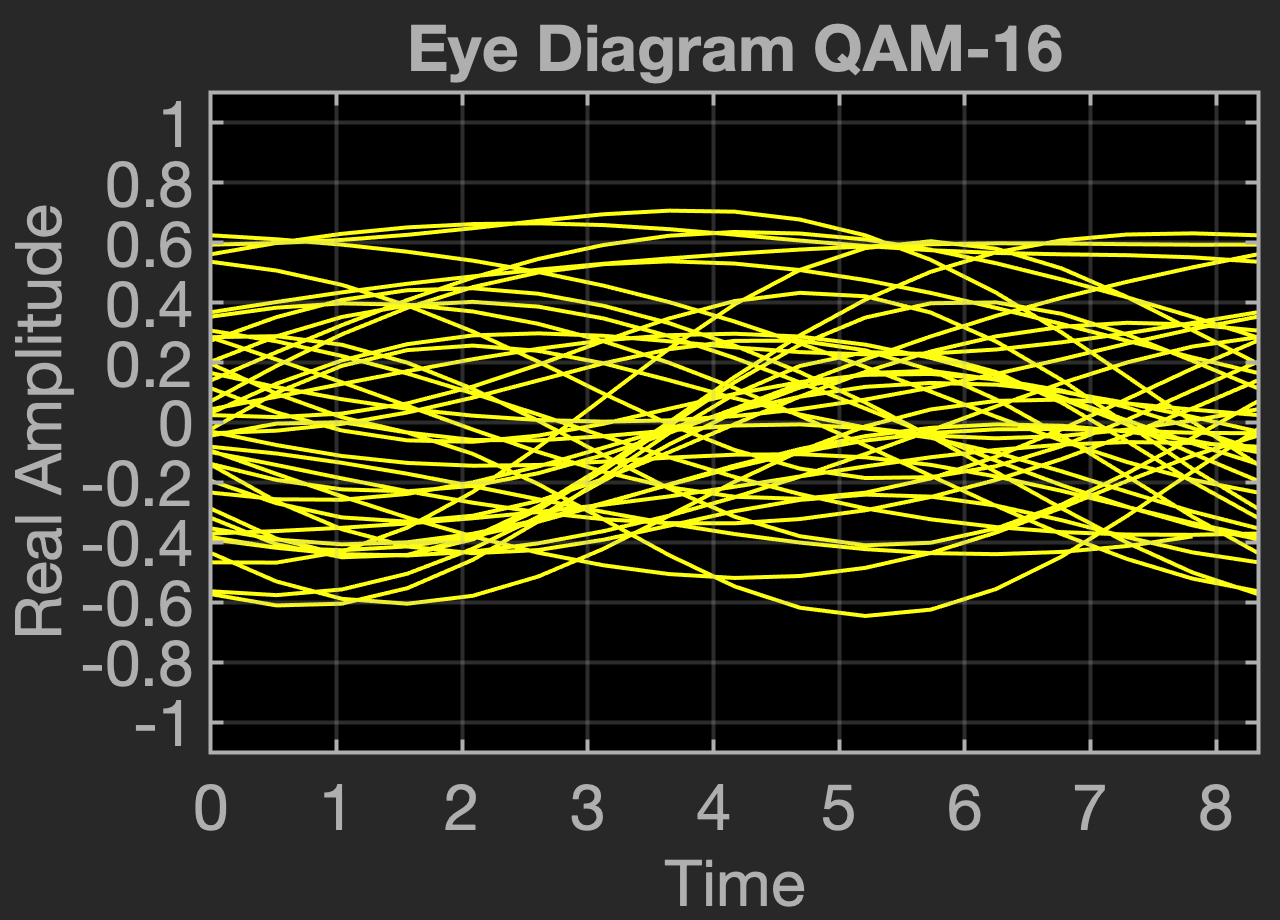
\includegraphics[width=0.45\linewidth]{eyeQAMgood.png}

}
  \caption{Eye diagram and constellation for QPSK (a and c) and QAM-16 (b and d) modulated symbols. Transmit power: \SI{\measPWR}{dBm}}
  \label{fig:good_diagrams} 
\end{figure}

% !TEX root = main.tex
\begin{figure} 
    \centering
  \subfloat[QPSK constellation\label{1a}]{%
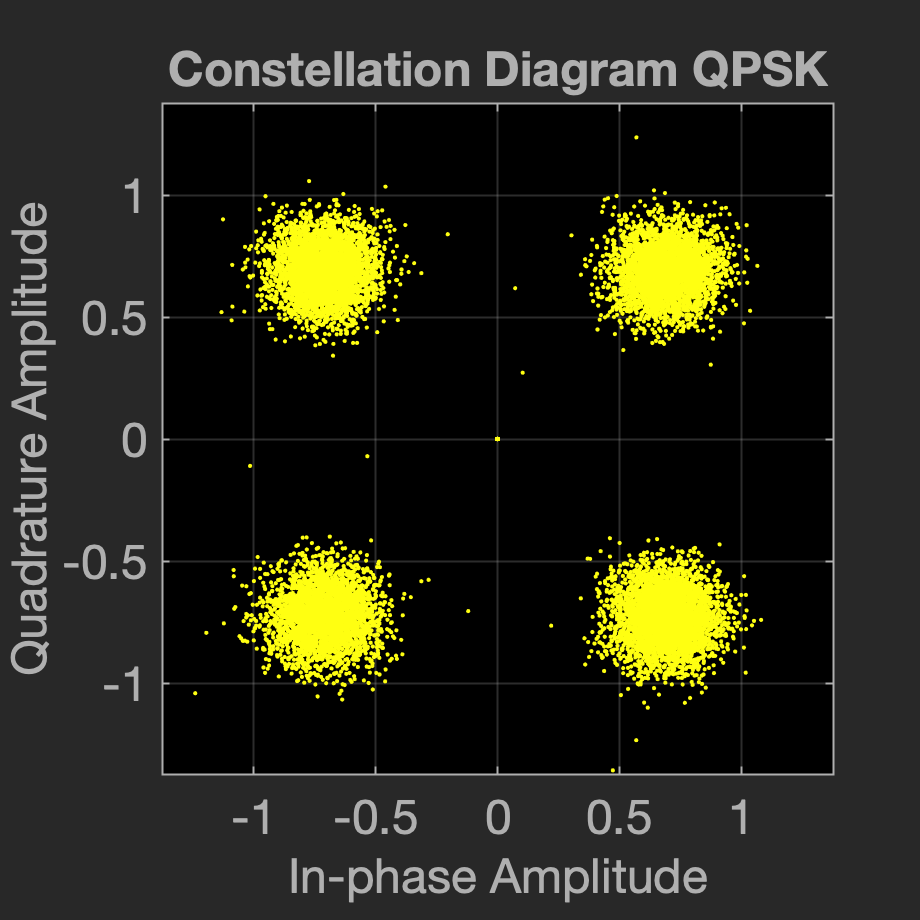
\includegraphics[width=0.45\linewidth]{constellationQPSKbad.png}
}
  \subfloat[QAM-16 constellation\label{1b}]{%
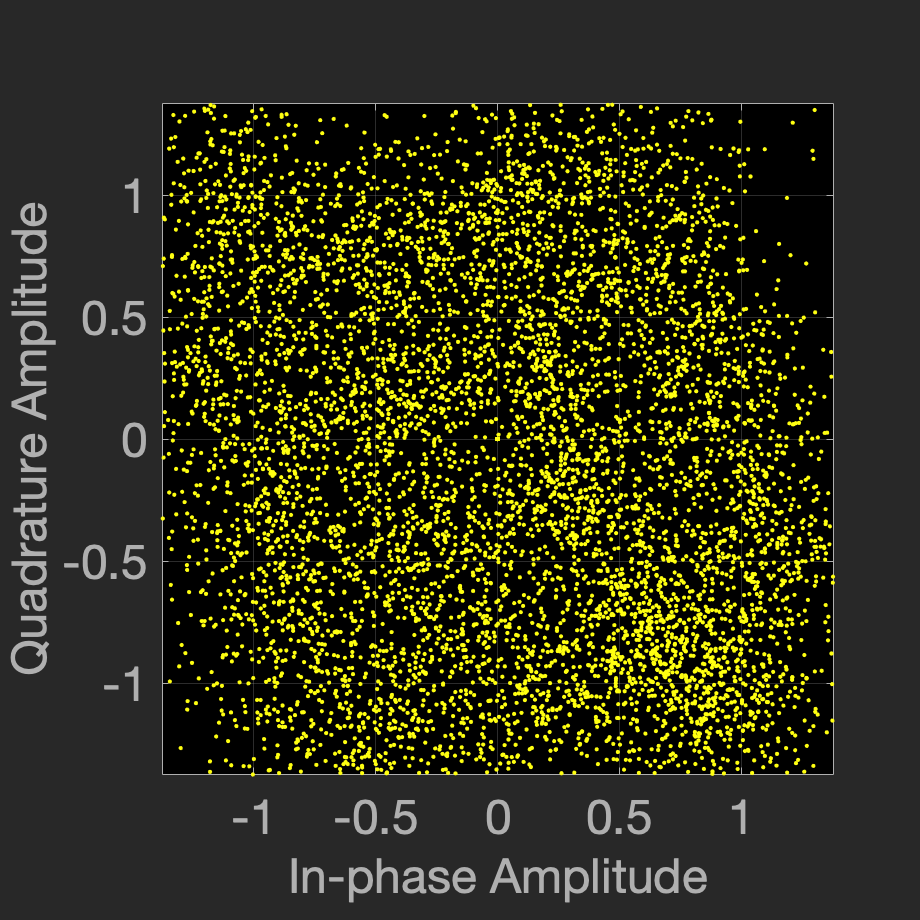
\includegraphics[width=0.45\linewidth]{constellationQAMbad.png}

}
\\
  \subfloat[QPSK eye diagram\label{1c}]{%
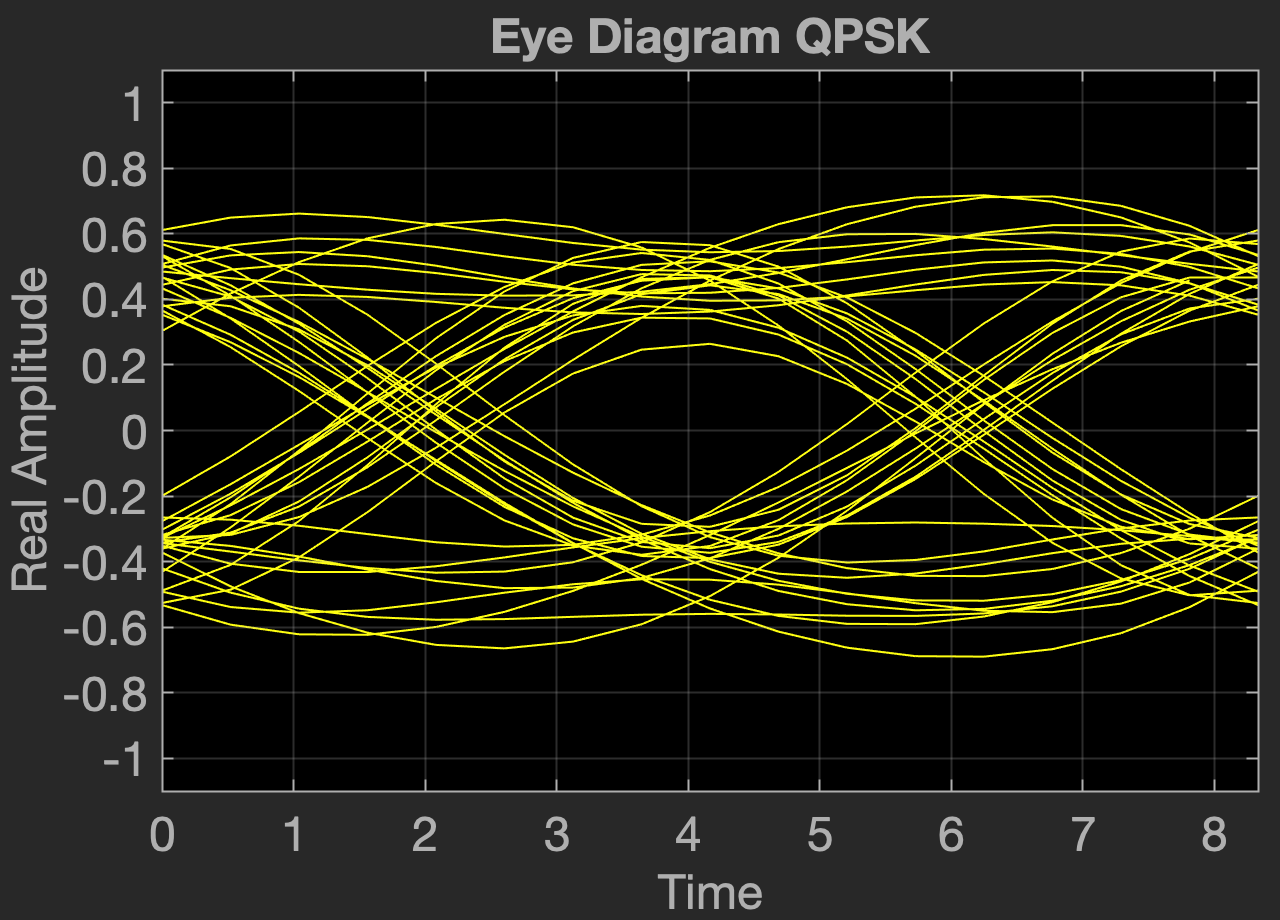
\includegraphics[width=0.45\linewidth]{eyeQPSKbad.png}

}
  \subfloat[QAM-16 eye diagram\label{1d}]{%
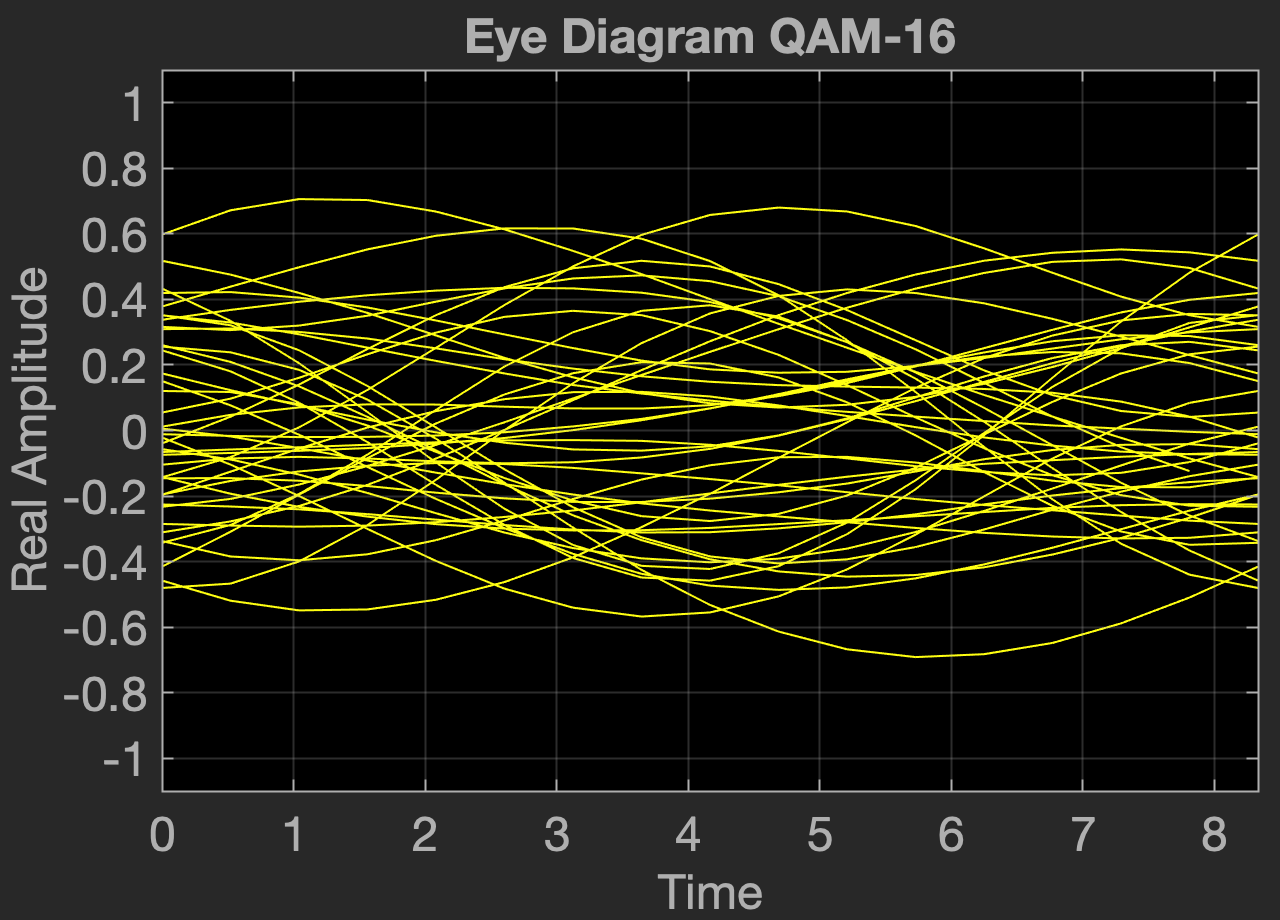
\includegraphics[width=0.45\linewidth]{eyeQAMbad.png}

}
  \caption{Eye diagram and constellation for QPSK (a and c) and QAM-16 (b and d) modulated symbols. Transmit power: $\measPWRbad \si{dBm}$}
  \label{fig:bad_diagrams} 
\end{figure}

% !TEX root = main.tex
\begin{table}[htbp]
  \centering
  \caption{Measured performance parameters. Transmit power: $\SI{\measPWR}{\decibel m}$}
    \begin{tabular}{lc}
    \rowcolor[rgb]{ 0,  0,  0} \textcolor[rgb]{ 1,  1,  1}{\textbf{System Parameter}}	& \textcolor[rgb]{ 1,  1,  1}{\textbf{Measured Value}} 		\\
    \rowcolor[rgb]{ 0,  0,  0} \textcolor[rgb]{ 1,  1,  1}{} & \textcolor[rgb]{ 1,  1,  1}{\textbf{Modulation QPSK / QAM-16}}					\\
    	SNR 													& $\SI{\measSNRQPSKGood}{dB} / \SI{\measSNRQAMGood}{dB}$							\\
	\ebnot 													& $\SI{13.1}{dB} /\SI{4.6}{dB}$							\\
    	BER			 											& \measBERQPSKGood / \measBERQAMGood 		\\
	EVM 													& $\SI{-17.5}{dB} / \SI{-14.5}{dB}$							\\

 \end{tabular}
  \label{tab:meas_params_good}
\end{table}
% !TEX root = main.tex
\begin{table}[htbp]
  \centering
  \caption{Measured performance parameters. Transmit power: $\measPWRbad \si{dBm}$}
    \begin{tabular}{lc}
    \rowcolor[rgb]{ 0,  0,  0} \textcolor[rgb]{ 1,  1,  1}{\textbf{System Parameter}}	& \textcolor[rgb]{ 1,  1,  1}{\textbf{Measured Value}} 		\\
    \rowcolor[rgb]{ 0,  0,  0} \textcolor[rgb]{ 1,  1,  1}{} & \textcolor[rgb]{ 1,  1,  1}{\textbf{Modulation QPSK / QAM-16}}					\\

    	SNR														& $\measSNRGood\si{dB}$						\\
    	EVM 													& $\measEVMGood \si{dB}$						\\
    	BER			 											& \measBERQPSKGood / \measBERQAMGood		\\
 \end{tabular}
  \label{tab:meas_params_bad}
\end{table}

Figure \ref{fig:ber_vs_snr} shows the measured BER as a function of estimated \ebnot. This value is compared to a theoretical BER (Estimated BER) to give an impression of the system performance under the given conditions. The BER is measured with $10^4$ frames of $1150$ bit each, making $8.7\cdot10^{-8}$ the smallest detectable BER. The estimated BER is based on white Gaussian noise only.
% !TEX root = main.tex
\begin{figure} 
    \centering
  \subfloat[QPSK \label{1a}]{%
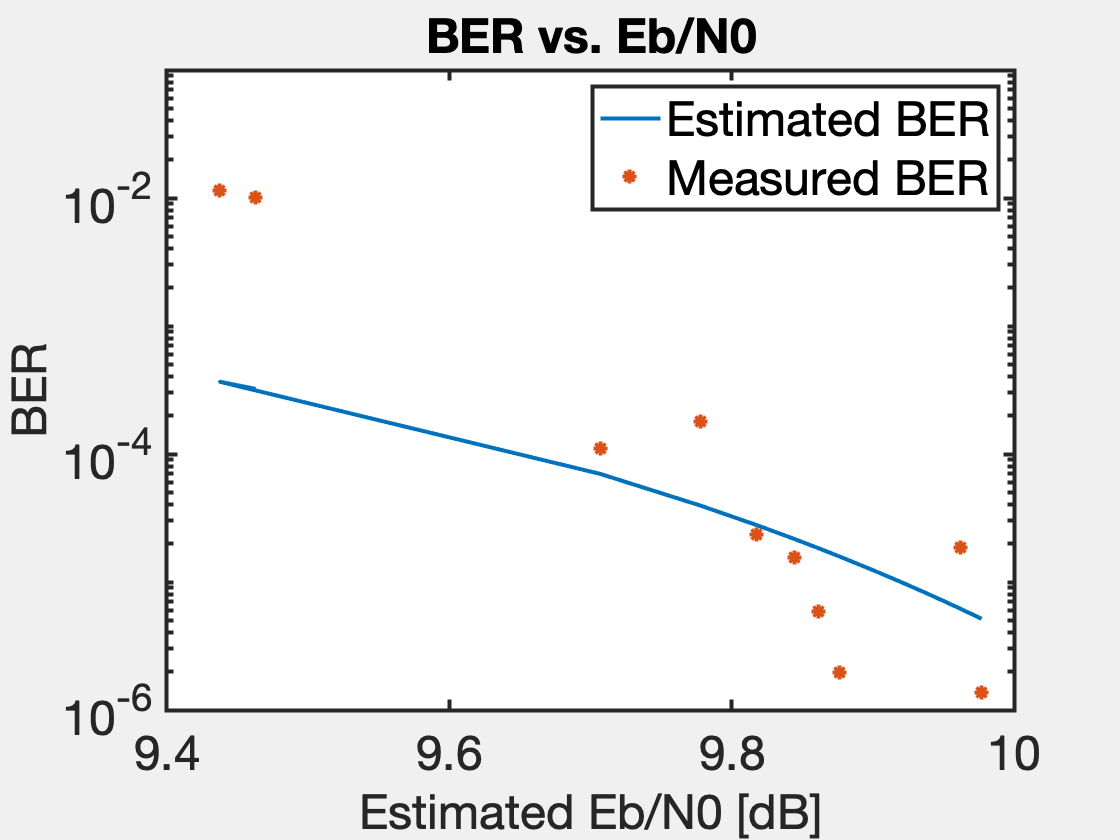
\includegraphics[width=0.45\linewidth]{BERvsSNRQPSK.png}
}
  \subfloat[QAM-16\label{1b}]{%
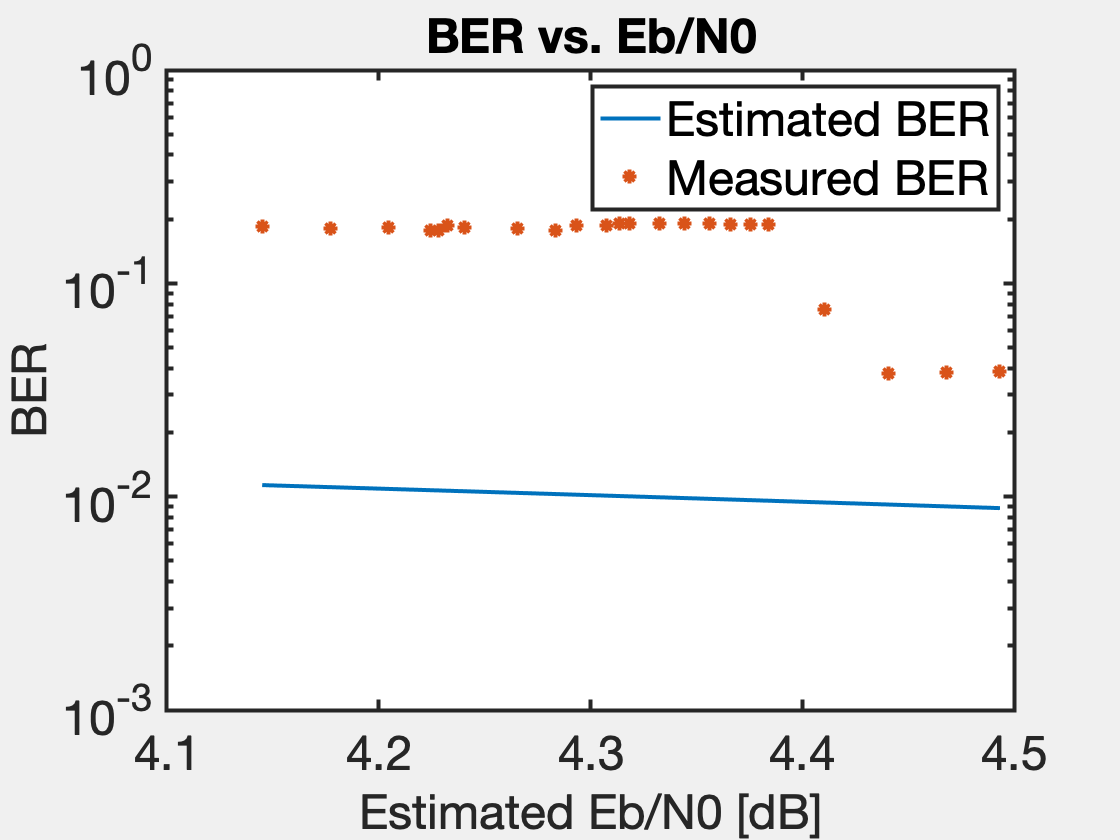
\includegraphics[width=0.45\linewidth]{BERvsSNRQAM.png}

}
  \caption{BER vs. SNR for both modulation formats. The estimated BER is the theoretical BER based on the estimated values for \ebnot and true BER is the actual calculated BER}
  \label{fig:ber_vs_snr} 
\end{figure}

\input{QAMBarker}

\subsection{Discussion of Obtained Results}
% Brief description of overall system performance
The proposed system is supposed to broadcast speech data with adaptable sound quality, by switching between QPSK and QAM-16 modulation based on the detected error rates. During the full system test, the threshold for changing state was set to \BERThreshold. With this threshold, the system changed quality state when the transmit power was reduced to about $\BERPowerLimit$ dBm. The test verified that the adaptable quality feature works as expected. The measured $\measDelay \si{ms}$ delay show that the system is well suited for two-way communication as well as broadcasting. 

% Short comment on power spectrum
Figure \ref{fig:pwr_spectrum} shows that the measured power spectrum lies very close to the theoretical spectrum. This indicates that the amount of nonlinear distortion introduced by the RF hardware is at a minimum.

% Short qualitative description of behaviour under QPSK modulation
When transmitting QPSK modulated data at low data rate, the system delivered almost noise free sound, at both power levels. The sound quality was not audibly reduced by the transmission. Figure \ref{fig:good_diagrams} and \ref{fig:bad_diagrams} and table \ref{tab:meas_params_good} and \ref{tab:meas_params_bad} supports this qualitative description. 

% Discussion of QAM-16 results
The transmission of QAM-16 modulated data was not equally successful. At the highest power level, the transmitted speech was barely audible. At the lowest power level the sound was completely lost in noise. This result is again supported by figure \ref{fig:good_diagrams} and \ref{fig:bad_diagrams} and table \ref{tab:meas_params_good} and \ref{tab:meas_params_bad}. The constellation diagram in figure \ref{fig:good_diagrams} (b) shows that the poor quality is mainly due to bad phase synchronization. Figure \ref{fig:QAMBarker} shows a comparison of the QAM-16 constellation with all frame symbols (a), and with the Barker symbols only (b). As the figure shows, the Barker symbols have no visible phase shift, which indicates that there is a phase difference between the Barker symbols and the rest of the frame. The reason for this problem is not understood by the authors and the issue remains for future improvements.

% Comment on BER vs Eb/N0 plot
The BER vs. \ebnot\ plots of figure \ref{fig:ber_vs_snr} gives an indication of how well the system performs under the given noise conditions, by comparing the measured BER to estimated BER, assuming white Gaussian noise only. For the QPSK modulated signal, the measured BER is higher than estimated for low \ebnot, and approaches the theoretical value as \ebnot increase. This is because the frequency and phase synchronization algorithms get less accurate as the noise level increase, which introduces more errors than what is obtained from AWGN only. For the QAM-16 modulation, the BER is constantly above the theoretical value, mostly because of the poor phase synchronization discussed previously. 



